\documentclass[mathserif]{beamer}
\DeclareMathSizes{10}{3}{3}{3}
\usepackage{graphicx} %The mode "LaTeX => PDF" allows the following formats: .jpg  .png  .pdf  .mps
\graphicspath{{./images/}} %Where the figures folder is located
\usepackage{media9}
\addmediapath{./videos/}
\usepackage{animate}
\usepackage{hyperref}
\usepackage{subcaption}
\usepackage{amsmath}
\usepackage{multicol}
\usepackage{paracol}
\usepackage[latin1]{inputenc}
\usetheme{fel}
\usepackage[scaled=0.45]{helvet}


\title{Scale separation in fast hierarchical solvers for discontinuous Galerkin methods}

\author[\underline{D. Kuzmin}, L. Korous, V. Aizinger]{Dmitri Kuzmin, Luk\' a\v s Korous, Vadym Aizinger}

\institute[Erlangen, Pilsen]{University Erlangen-N\"urnberg, University of West Bohemia} 
\begin{document}

\newcommand{\bs}[1]{\LARGE \textit{\textbf{#1}}}

\newcommand{\D}{\mathrm{d}}
\newcommand{\pd}[2]{\frac{\partial #1}{\partial #2}}
\newcommand{\msc}[1]{\mbox{\sc #1}}
\newcommand{\mschat}[1]{\hat{\mbox{\sc #1}}}
\newcommand{\mbf}[1]{\mbox{\small$\mathbf{#1}$}}
\newcommand{\mbfhat}[1]{\mbox{\small$\hat{\mathbf{#1}}$}}
\newcommand{\dx}{\,\mathrm{d}\mathbf{x}}
\newcommand{\ds}{\,\mathrm{d}s}
\newcommand{\be}{\begin{equation}}
\newcommand{\ee}{\end{equation}}
\newcommand{\bea}{\begin{eqnarray}}
\newcommand{\eea}{\end{eqnarray}}
\newcommand{\bn}{\mathbf{n}}
\newcommand{\bx}{\mathbf{x}}
\newcommand{\ba}{\mathbf{a}}
\newcommand{\bv}{\mathbf{v}}
\newcommand{\bu}{\mathbf{u}}
\newcommand{\bb}{\mathbf{b}}
\newcommand{\ff}{\mathbf{f}}
\newcommand{\p}{\partial}


% Total derivative
\newcommand{\td}[2]{\frac{\D #1}{\D #2}}

\newcommand{\jump}[1]{[\![#1]\!]}


\begin{frame}
\large
\titlepage
\end{frame}

\section{Introduction}
\subsection{Current state-of-the-art in solving linear systems originating from DG discretization}

\begin{frame}

We are concerned with solving linear problems that arise from DG discretization\ \\
Most improvements over a general approach (generic matrix solver) use some variation of the p-multigrid scheme:

\begin{itemize}
\item \vspace{-2mm} K. Hillewaert, J.-F. Remacle, N. Cheveaugeon, P.-E. Bernard, and P. Geuzaine\\
 \vspace{-2.5mm} Analysis of a hybrid p-multigrid method for the Discontinuous Galerkin Discretisation of the Euler Equations.

\item \vspace{-2mm} H. Luo, J.D. Baum, and R. L\"ohner\\
\vspace{-2.5mm} Fast p-multigrid discontinuous Galerkin method for compressible flows at all speeds.

\item \vspace{-2mm} F. Bassi, A. Ghidoni, S. Rebay, P. Tesini\\
\vspace{-2.5mm} High-order accurate pmultigrid discontinuous Galerkin solution of the Euler equations.

\item \vspace{-2mm} R. Nastase and D. J. Mavriplis\\
\vspace{-2.5mm} High-order discontinuous Galerkin methods using an hp-multigrid approach.

\end{itemize}

These approaches (as well as our method) work especially well if the DG discretization uses a hierarchical basis.
\end{frame}


\subsection{Overview of our proposed method - HSS}


\begin{frame}

The hierarchical scale separation (HSS) technique explored in this work
differs from the p-multigrid method in two key aspects:
\begin{enumerate}
\item instead of using a full hierarchy of approximations as smoothers we only need two approximations, coarse and fine, for a DG scheme of any order
\item our fine scale smoothing does not affect any coarse degrees of freedom resulting in a more complete decoupling of the coarse and fine-scale problems
\end{enumerate}

Steps:\ \\

\begin{enumerate}
\item The coarse-scale problem solves for cell \textbf{mean values} and has the computational structure of a cell-centered finite volume method.
\item The \textbf{local} fine-scale problems are solved using the fluxes that contain the results of the global coarse-scale solve.
\end{enumerate}

\end{frame}

\subsection{Benefits of our proposed method - HSS}
\begin{frame}
\begin{enumerate}
\item {\large \textbf{Easy parallelization}}\ \\
In contrast to the full p-multigrid algorithm, all fine-scale components associated with the same element are updated simultaneously.

\item {\large \textbf{Natural implementation of flux limiting}}\ \\
As the algorithm is divided into calculation of mean values and the higher degree part (which needs to be limited in the case of shocks appearing in the solution), it is easy to plug in flux limiting to the part which updates the derivatives.
\end{enumerate}

\end{frame}

\small

\subsection{Model problem}
\begin{frame}
\begin{equation}
\frac{\p u}{\p t}
+\nabla\cdot(\ba u) + D \Delta u =0
\qquad\mbox{in}\ \Omega,\label{goveq}
\end{equation}
where
\begin{itemize}
\item $\Omega$ is a bounded domain
\item $u(\bx,t)$ is a conserved scalar quantity
\item $\ba(\bx,t)$ is a (continuous) velocity field
\item $D(\bx,t)$ a diffusivity coefficient.
\end{itemize}
In the present work, we consider several limiting cases of the above equation: 
pure convection, convection-dominated, and diffusion-dominated. 
In addition, the stationary problem $\left(\frac{\p u}{\p t}=0\right)$ was tested for all three settings.

\end{frame}


\subsection{Model problem - boundary conditions}
\begin{frame}

The initial condition is given by $u(\cdot,0)=u_0\qquad\mbox{in}\ \Omega$.\ \\

\begin{itemize}
\item The inflow boundary is defined as $\Gamma_{\rm in}=\{\bx\in\Gamma\,|\, \ba(\bx, t)\cdot\bn(\bx)<0\}$, where $\bn$ denotes the unit outward normal to the boundary $\Gamma=\p\Omega$.
\item Similarly, we call $\Gamma_{\rm out}=\{\bx\in\Gamma\,|\, \ba(\bx, t)\cdot\bn(\bx) \ge 0\}$ the outflow boundary.
\item The Dirichlet boundary condition $ u=u_{\rm in} \mbox{ on } \Gamma_{\rm in} \label{dbc}$ is imposed for pure convection ($D=0$) and convection-diffusion problems.
\\ \hspace{5mm}If $D>0$ we enforce, in addition, $u=u_{\rm out} \mbox{ on } \Gamma_{\rm out} \label{dbc2}$.
\end{itemize}
\end{frame}

\subsection{Notation}
\begin{frame}

We call ${\cal T}_h$ a (possibly unstructured) computational mesh 
and ${\cal S}_h$ will denote the set of all internal edges/faces in ${\cal T}_h$.\ \\
On the interface between elements $K^+\in{\cal T}_h$ and $K^-\in{\cal T}_h$,
the traces are given by the one-sided limits
\vspace{-2mm}
$$
u^\pm(\bx,t)=\lim\limits_{\epsilon\to + 0}u(\bx
-\mathbf{\epsilon}\bn^{\pm},t),\quad \bx\in\p K,
$$
\vspace{2mm}
where $\bn^{\pm}$ are the external unit normals to $K^{\pm}$.\ \\
\vspace{-2mm}
The mean and the jump of a scalar $u$ across the common boundary of $K^+$
and $K^-$ are denoted by
\vspace{-3mm}
\[
\{u(\bx, t)\} = \frac 12 \left( u^+(\bx, t) + u^-(\bx, t) \right)
\]
\vspace{-6mm}
\[
\jump{u(\bx, t)} =  u^+(\bx, t) \; \bn^+(\bx) + u^-(\bx, t) \; \bn^-(\bx) 
\]
respectively.
Similarly, the mean and the jump of a vector $\bv$ are given by
\vspace{-3mm}
\[
\{\bv(\bx, t)\} = \frac 12 \left( \bv^+(\bx, t) + \bv^-(\bx, t) \right)
\]
\vspace{-6mm}
\[
\jump{\bv(\bx, t)} = 
\bv^+(\bx, t) \cdot \bn^+(\bx) + \bv^-(\bx, t) \cdot \bn^-(\bx).
\]
In this context, one has to keep in mind that jumps of scalars are vectors, whereas 
jumps of vectors are scalar quantities.
\end{frame}



\subsection{Discrete formulation}

\begin{frame}
We consider an arbitrary internal element $K\in {\cal T}_h$.\ \\
Here we use the nonsymmetric interior penalty Galerkin (NIPG) formulation for the second-order terms
\bea
\hspace{-8mm}\int_{K}w\pd{u}{t} \dx 
&-& \int_{K}\nabla w\cdot\ba\; u \dx
+\int_{\p K} w\; \ba \cdot \bn \; \hat u \; ds
+ \int_{K} D \nabla u \cdot \nabla w \dx \nonumber \\
&-&\int_{\p K} D \left(w \{\nabla u\}
- \{\nabla w \} u 
- \sigma w \jump{u} \right) \cdot \bn \ds \;=\;0, \quad
\forall w\in V,  \nonumber
\eea
\begin{itemize}
\item $V$ is the space of admissible test functions
\item \vspace{-1mm} $\hat u$ is the upwind-sided trace of the (generally discontinuous) function
\begin{itemize}
\item \vspace{-1mm} $u:\Omega\to\mathbb{R}$
\end{itemize}
\item \vspace{-1mm} $\sigma$ is the penalty coefficient usually chosen as
\begin{itemize}
\item \vspace{-1mm} $\sigma=O(1/h_K)$
\end{itemize}
\item \vspace{-1mm} $h_K$ is the size of element $K$.
\end{itemize}

\end{frame}



\subsection{Discrete formulation - boundary conditions}

\begin{frame}
The inflow and outflow boundaries of element $K$
are defined by
$$
\p K_{\rm in}=\{\bx\in\p K\,|\, \ba(\bx, t)\cdot\bn(\bx)<0\},$$
$$
\p K_{\rm out}=\{\bx\in\p K\,|\, \ba(\bx, t)\cdot\bn(\bx)\ge0\}.$$
By virtue of (\ref{dbc}), we have  $\hat u=u_{\rm in}$ on $\p K_{\rm in}\cap \Gamma_{\rm in}$.\ \\
Selecting the upwind-sided value (we associate here $K$ with $K^-$), 
we define the convective fluxes using
\begin{equation}
\hat u(\bx,t)=\left\{\begin{array}{rl}
u^+(\bx,t)&\quad\mbox{if} \ \bx\in\p K_{\rm in}\backslash\Gamma_{\rm in},\\ 
u_{\rm in}(\bx,t) &\quad\mbox{if} \ \bx\in\p K_{\rm in}\cap\Gamma_{\rm in},\\
u^-(\bx,t)&\quad\mbox{otherwise}.
\end{array}\right.
\label{upw}
\end{equation}
In the parabolic case ($D>0$), we associate the values of $\hat u^+$ on the exterior boundaries with the specified Dirichlet boundary conditions:
\begin{equation}
\hat u^+(\bx,t)=\left\{\begin{array}{rl}
u^+(\bx,t)&\quad\mbox{if} \ \bx\in\p K\backslash\p \Omega,\\ 
u_{\rm in}(\bx,t) &\quad\mbox{if} \ \bx\in\p K\cap\Gamma_{\rm in},\\
u_{\rm out}(\bx,t) &\quad\mbox{if} \ \bx\in\p K\cap\Gamma_{\rm out}.
\end{array}\right.
\label{diff}
\end{equation}

\end{frame}




\subsection{Local problem}
\begin{frame}
Writing the local problem for an element $K$ we obtain
\begin{equation}
\left(w,\pd{u}{t}\right)_K+a_K(w,u)=b_K(w),\qquad \forall w\in V,
\label{weakloc}
\end{equation}
where
\begin{eqnarray}
a_K(w,u)&=&\int_{K}\left( D \nabla u \cdot \nabla w 
\;-\; \nabla w\cdot\ba \; u \right)\dx
+\int_{\p K_{\rm out}} w \; u \; \ba\cdot\bn\ds \nonumber\\
&&-\int_{\p K} D \left( \frac 12 w \nabla u \cdot \bn
- \frac 12 \; \nabla w \cdot \bn \; u - \sigma \; w \; u \right)\ds, \label{loc1}\\
b_K(w)&=&-\int_{\p K_{\rm in}} w\; \hat u\; \ba\cdot\bn\ds \nonumber\\
&&+\int_{\p K} D \left(\frac 12 \; w \; \nabla \hat u^+ \cdot \bn
- \frac 12 \; \nabla w \cdot \bn \; \hat u^+ 
+ \sigma \; w \; \hat u^+ \right)\ds, \hspace{8mm}\label{loc2}\\
\left(w,\pd{u}{t}\right)_K&=&
\int_{K}w\; \pd{u}{t}\; \dx.\label{loc3}
\end{eqnarray}

\end{frame}




\subsection{Global semi-discrete problem}
\begin{frame}


After summation over all elements in ${\cal T}_h$ one arrives at the global 
semi-discrete problem given by
\begin{equation}
\left(w,\pd{u}{t}\right)+a(w,u)=b(w),\qquad \forall w\in V,
\label{weakglob}
\end{equation}
where
\begin{eqnarray}
a(w,u)&=&\sum_{K\in {\cal T}_h}\int_{K}\left( D \nabla u \cdot \nabla w 
\;-\; \nabla w \; \cdot\ba \; u \; \right)\dx\nonumber\\
&&+\int_{\Gamma_{\rm out}} w \; u \; \ba\cdot\bn\ds 
+\sum_{S\in {\cal S}_h}\int_{\p K} \hat u \; \ba \cdot \jump{w}\nonumber\\
&&-\sum_{S\in {\cal S}_h}\int_{\p K} D \left(\{\nabla u\} \jump{w}
- \{\nabla w \} \jump{u} 
- \sigma \jump{w} \jump{u} \right) \ds\nonumber\\
&&-\int_{\p \Omega} D \left(w \nabla u \cdot \bn - \frac 12 \; u \nabla w \cdot \bn 
- \sigma \; w \; u \right) \ds, \label{glob1}\\
b(w)&=-&\int_{\Gamma_{\rm in}} \left\{ w \; u_{\rm in} \; \ba\cdot\bn
- D \left(\frac 12 \; u_{\rm in} \nabla w \cdot \bn 
+ \sigma \; w \; u_{\rm in}  \right) \right\}\ds\nonumber\\
&&+\int_{\Gamma_{\rm out}} D \left(\frac 12 \; u_{\rm out} \nabla w \cdot \bn 
- \sigma \; w \; u_{\rm out}  \right) \ds,\label{glob2}\\
\left(w,\pd{u}{t}\right)&=&\sum_{K\in {\cal T}_h}\int_{K}w\; \pd{u}{t}\; \dx.
\label{glob3}
\end{eqnarray}
\end{frame}




\begin{frame}
Now
\begin{itemize}
\item we replace the space of weak solutions $V$ with its finite-dimensional counterpart $V_h$.
\item In the case of a DG method, it consists of piecewise polynomials defined on elements $K\in {\cal T}_h$ with no global continuity requirements. 
\item The restriction of the numerical solution $u_h$ to an element $K\in {\cal T}_h$ is then given by $u_h(\bx,t)=\sum_ju_j(t)\varphi_j(\bx),\qquad\bx \in K\label{approx}$.
\end{itemize}
For functions from $V_h$, the local problem (\ref{weakloc}) becomes 
\begin{equation}
\left(w_h,\pd{u_h}{t}\right)_K+a_K(w_h,u_h)=b_K(w_h),\qquad 
\forall w_h\in V_h.
\label{weakloc2}
\end{equation}
By (\ref{approx}), this variational problem is equivalent to the linear system
\begin{equation}
\sum_j\td{u_i}{t}
\left(\varphi_i,\varphi_j\right)_K
+\sum_ju_ja_K(\varphi_i,\varphi_j)=
b_K(\varphi_i),\qquad \forall i.
\label{weakloc_h}
\end{equation}
\end{frame}



\subsection{The matrix form}
\begin{frame}

The matrix form of the so-defined semi-discrete 
local problem reads
\begin{equation}
M_K\td{\bu_K}{t}+A_K \bu_K=\ff_K,\label{discrloc}
\end{equation}
where $\displaystyle \bu_K$ is the local vector of degrees of freedom corresponding to element $K$, 
$\displaystyle M_K=\{m_{ij}\}$ is the element mass matrix, 
$\displaystyle A_K=\{a_{ij}\}$ is the discrete convection-diffusion operator 
(including the outgoing fluxes), and $\displaystyle \ff_K=\{f_i\}$ is the vector of 
incoming fluxes. By (\ref{weakloc_h}), the coefficients are given by
\begin{equation}
m_{ij}=(\varphi_i,\varphi_j)_K,
\end{equation}
\begin{equation}
a_{ij}=a_K(\varphi_i,\varphi_j),
\end{equation}
\begin{equation}
f_i=b_K(\varphi_i).
\end{equation}
The global system can be assembled from element contributions which
are coupled through the surface integrals in the
coefficients $a_{ij}$ and $f_i$. 
\end{frame}



\subsection{Taylor basis functions}

\begin{frame}
In multi-index notation with $p=(p_1, p_2, \dots, p_d)$, we define the Taylor basis functions on element $K$ as
\be
\varphi^{(0)}_K(\bx)=1, \qquad 
\varphi^{(p)}_K(\bx)=\frac{(\bx-\bx_0)^p-\overline{(\bx-\bx_0)}^p}{p!\Delta \bx^p},
\label{phidef}
\ee
where the scaling $\Delta \bx = (\frac{x_{1, \max}-x_{1, \min}}2, 
\frac{x_{2, \max}-x_{2, \min}}2, \dots, \frac{x_{d, \max}-x_{d, \min}}2)$ 
is given by a vector describing the half-size of the smallest $d$-dimensional slab 
containing element $K$.\ \\
This purpose of this scaling is to improve the conditioning of the mass matrix 
arising from the Taylor basis discretization.\ \\

Equation (\ref{approx}) can be now written as 
\begin{equation}
u_h(\bx,t)=\sum_{0 \le |p| \le k} u^{(p)}_K(t)\varphi^{(p)}_K(\bx),\qquad
\bx \in K
\end{equation}
with
\be
u^{(0)}_K = \bar{u}_h{\big|_K}, \qquad u^{(p)}_K=D^pu_h(\bx_0) \Delta\bx^p,
\quad |p|>0.
\ee
\end{frame}




\section{Hierarchical scale separation}
\subsection{Separation to mean values and derivatives}

\begin{frame}
Hierarchical bases, such as Taylor basis functions, naturally accommodate 
decompositions of the local DG approximation such as
\begin{equation}
u_h=\bar u_h+u_h',
\end{equation}
where $u_h'=u_h-\bar u_h$ is the contribution of higher order 
(e.g., linear, quadratic) terms in (\ref{approx}). 

The Taylor basis functions associated with $\bar u_h$ and $u_h'$
are given by $\{\varphi_1\}$ and  $\{\varphi_i, \; i\ge2\}$,
respectively. The space of test functions admits a similar
decomposition. Thus, the local problem can be
split into two subproblems
\bea
\hspace{-12mm}&\left(\bar w_h,\pd{\bar u_h}{t}+\pd{u_h'}{t}\right)_K &
+\;a_K(\bar w_h,\bar u_h+u_h')
\;=\;b_K(\bar w_h), \; \forall 
\bar w_h \in \mbox{span}\{\varphi_1\},\label{loc1vms}\\
\hspace{-12mm}&\left(w_h',\pd{\bar u_h}{t}+\pd{u_h'}{t}\right)_K&
+\;a_K(w_h',\bar u_h+u_h')
\;=\;b_K(w_h'), \; \forall w'_h
\in \mbox{span}\{\varphi_{i, i \ge 2}\}.\label{loc2vms}
\eea
\end{frame}


\subsection{Separation to mean values and derivatives - Global systems}
\begin{frame}
Summing over all elements $K\in {\cal T}_h$ and rearranging the terms, 
we can write the global system defined in (\ref{loc1vms}), (\ref{loc2vms}) 
in matrix form as
\begin{eqnarray}
\vspace{-2mm}
\begin{bmatrix}
  \bar{M} & 0 \\  0 & M'
 \end{bmatrix} 
\frac d{d t}
\begin{bmatrix}
  \bar{\bu} \\  \bu'
 \end{bmatrix} 
\; + \;
\begin{bmatrix}
  \overline{A} & \overline{B} \\  B' & A'
 \end{bmatrix}
\begin{bmatrix}
  \bar{\bu} \\  \bu'
 \end{bmatrix}
\;=\;
\begin{bmatrix}
  \bar{\bb} \\  \bb'
 \end{bmatrix},
\vspace{-2mm}
\end{eqnarray}

where $\bar{\bu}, \bu'$ are the global vectors of unknowns associated with the coarse-
and the fine-scale parts of the solution, respectively.\ \\
The remaining matrices and vectors are defined as follows:
\vspace{-2mm}
\begin{align*}
&\overline{M} = \left(\varphi_{K, 1}, \varphi_{L, 1}\right)_{K, L \in {\cal T}_h},
&& M'=\left(\varphi_{K, j},  \varphi_{L, i}\right)_{K, L \in {\cal T}_h,\; i, j \ge 2},\\
&\overline{A} = a(\varphi_{K, 1}, \varphi_{L, 1})_{K, L \in {\cal T}_h}, 
&& \overline{B} = a(\varphi_{K, 1}, \varphi_{L, i})_{K, L \in {\cal T}_h,\; i \ge 2},\\
&A' = a(\varphi_{K, j},  \varphi_{L, i})_{K, L \in {\cal T}_h,\; i, j \ge 2},
&& B' = a(\varphi_{K, j}, \varphi_{L, 1})_{K, L \in {\cal T}_h,\; j \ge 2},\\
&\bar \bb = b(\varphi_{K, 1})_{K \in {\cal T}_h},
&& \bb' = b(\varphi_{K, j})_{K \in {\cal T}_h, \; j \ge 2}
\end{align*}

with $\varphi_{K, i}$ denoting the Taylor basis functions on element $K \in {\cal T}_h$.\ \\
In order to decouple the inter-element dependencies of the fine scales, we decompose the matrix $A'$ into
\begin{itemize}
\vspace{-2mm}
\item the block-diagonal part $\tilde{A}'$ 
\vspace{-2mm}
\item the remainder $A'-\tilde{A}'$.
\end{itemize}
\end{frame}



\subsection{The algorithm}
\begin{frame}
Without loss of generality we discretize the semi-discrete problem
in time using the backward Euler scheme. 
Then, for a given vector of unknowns $\bu^n$ corresponding to time level $n$, 
 one cycle of the HSS method is given by:\\
\[\hspace{-9.1cm}\;\; \bu^{(0)}=\bu^n, \; k=0\]
{\it while $\bu^{(k)}$ not converged}
\begin{enumerate}
\item
$\displaystyle
\left(\frac{M'}{\Delta t} + \tilde{A}'\right) \tilde{\bu}'^{(k+1)}
= \frac{M'}{\Delta t} \begin{Bmatrix} \bu'^n \\ \bu'^{(k)} \end{Bmatrix}
- B' \bar \bu^{(k)} - \left(A'-\tilde{A}'\right) \bu'^{(k)} +\bb'
$
\item
$\displaystyle
\left(\frac{\overline{M}}{\Delta t} + \overline{A}\right) \bar \bu^{(k+1)} 
= \frac{\overline{M}}{\Delta t} \begin{Bmatrix} \bar \bu^n\\ \bar \bu^{(k)} \end{Bmatrix}
- \overline{B} \tilde{\bu}'^{(k+1)} + \bar \bb
$
\item
$\displaystyle
\left(\frac{M'}{\Delta t} + \tilde{A}'\right) \bu'^{(k+1)}
= \frac{M'}{\Delta t} \begin{Bmatrix} \bu'^n \\ \bu'^{(k)} \end{Bmatrix}
- B' \bar \bu^{(k+1)} - \left(A'-\tilde{A}'\right) \tilde{\bu}'^{(k+1)} +\bb'
$
\item
$\displaystyle
\bu^{(k+1)} = \bar \bu^{(k+1)} + \omega \bu'^{(k+1)} +(1-\omega)\bu'^{(k)}
$
\item
$\displaystyle
k = k+1
$
\end{enumerate}
{\it end while}
\[\hspace{-9.5cm}\;\; \bu^{n+1}=\bu^{(k)}\],
where $\omega \in (0, 1]$ is an under-relaxation parameter used to improve 
the convergence behavior in steady-state computations.
\end{frame}


\section{p-Multigrid implementation to compare with}
\subsection{Overview}

\begin{frame}
Given $\displaystyle k_1, k_2$, the numbers of pre-/postsmoothing iterations, the lower 
index $p\in \{0,1,2\}$ denotes the $p$-level of the algorithm. Similarly to the HSS method, 
$\tilde{A}$ stands for the block-diagonal part of 
the matrix $A$. If we denote by $\text{P}^p(K)$ the space of polynomials of degree less 
or equal to $p$ on element $K$, the mass matrix at the corresponding $p$-level is given by
\[
M_p=\left(\varphi_{K, j},  \varphi_{L, i}\right)_{K, L \in {\mathcal T}_h,\; 
\varphi_{L, i} \in \text{P}^p (L), \varphi_{K, j} \in \text{P}^p (K)}.
\]
with similar expressions for other matrices and vectors. 
The restriction $I_i^j$ and prolongation $J_j^i$ operators are represented by 
the $L^2$-projections between polynomial spaces corresponding to the $i$- and $j$-levels.
\end{frame}

\begin{frame}
\renewcommand{\thefootnote}{$\star$} 
{\it Algorithm($p$-multigrid):} 
\vspace{2mm}
\[
\hspace{-9.1cm}\;\; \bu_2^{(0)}=\bu^n,\; k=0
\]
{\it while $\bu_2^{(k)}$ not converged}
\begin{enumerate}
\item Presmoothing on level 2, which yields $\bu_{2}^{(k+k_1)}$
\item Presmoothing on level 1, which yields $\bu_1^{(k+k_1)}$
\item Solution on level 0, which yields $\bu_0^{(k+1)}$
\item Postmoothing on level 1, which yields $\bu_1^{(k+k_1+k_2)}$
\item Postmoothing on level 2, which yields $\bu_2^{(k+k_1+k_2)}$
\item $\displaystyle k=k+k_1+k_2$
\end{enumerate}
{\it end while}
\[
\hspace{-9.9cm}\;\; \bu^{n+1}=\bu_2^{(k)}.
\]



\end{frame}

\subsection{Presmoothing on level 2}
\begin{frame}
{\Large Presmoothing on level 2 $\star$}
for $i = 0, \dots , k_1-1$ do:
\[
\left(\frac{M_2}{\Delta t} + \tilde{A}_2\right) \bu_2^{(k+i+1)} 
= \frac{M_2}{\Delta t} \begin{Bmatrix} \bu^n\\ \bu_2^{(k+i)} \end{Bmatrix} 
- \left(A_2-\tilde{A}_2\right) \bu_2^{(k+i)} + \bb_2,
\]
which yields $\bu_{2}^{(k+k_1)}$.\ \\\ \\
All smoothing and 
solution operators can be re-formulated using 
the residual/correction notation commonly used in the theory of multigrid
methods. E.g., the equation in step 1:
$$\left(\frac{M_2}{\Delta t} + \tilde{A}_2\right) 
\left(\bu_2^{(k+i+1)} - \bu_2^{(k+i)}\right) 
= \frac{M_2}{\Delta t}\left( \bu^n-\bu_2^{(k+i)}\right) + \bb_2 - A_2\bu_2^{(k+i)}$$

% The residual reads:
% \[
% r_2 = \bb_2 - A_2 \bu_{2}^{(k+k_1)}
% \]
\end{frame}


\subsection{Presmoothing on level 1}
\begin{frame}
{\Large Presmoothing on level 1}
\begin{eqnarray*}
\bu_1^{(k)} & = & I_2^1\left(\bu_2^{(k+k_1)}\right)\\
\ff_1 & = & A_1 I_2^1\left(\bu_2^{(k+k_1)}\right) - I_2^1 \left(A_2 \bu_2^{(k+k_1)} \right)
\end{eqnarray*}
for $i = 0, \dots, k_1-1$ do:
\[
\left(\frac{M_1}{\Delta t} + \tilde{A}_1\right) \bu_1^{(k+i+1)}
= \frac{M_1}{\Delta t} \begin{Bmatrix} I_2^1 \bu^n\\\bu_1^{(k+i)} \end{Bmatrix} 
- \left(A_1-\tilde{A}_1\right) \bu_1^{(k+i)} + \bb_1 + \ff_1,
\]
which yields $\bu_1^{(k+k_1)}$.
%  The residual reads:
% \[
% r_1 = \bb_1 - A_1 \bu_{1}^{(k+k_1)}
% \]

\end{frame}


\subsection{Solution on level 0}
\begin{frame}
{\Large Solution on level 0}
\begin{eqnarray*}
\bu_0^{(k)} & = & I_1^0\left(\bu_1^{(k+k_1)}\right)\\
\ff_0 & = & A_0 I_1^0\left(\bu_1^{(k+k_1)}\right) - I_1^0\left(A_1 \bu_1^{(k+k_1)}\right) + I_1^0 \ff_1
\end{eqnarray*}
Solve 
\[
\left(\frac{M_0}{\Delta t} + A_0\right) \bu_0^{(k+1)}
=  \frac{M_0}{\Delta t} \begin{Bmatrix} I_2^0 \bu^n\\\bu_0^{(k)} \end{Bmatrix} + \bb_0 + \ff_0,
\]
which yields $\bu_0^{(k+1)}$.
\end{frame}


\subsection{Postsmoothing on level 1}
\begin{frame}
{\Large Postsmoothing on level 1}
\[
\bu_1^{(k+k_1)} = J_0^1 \bu_0^{(k+1)} - J_0^1\left(I_1^0 \bu_1^{(k+k_1)}\right) + \bu_1^{(k+k_1)}
\]
for $i = 0, \dots, k_2-1$ do:
\[
\left(\frac{M_1}{\Delta t} + \tilde{A}_1\right) \bu_1^{(k+k_1+i+1)} 
= \frac{M_1}{\Delta t} \begin{Bmatrix} I_2^1 \bu^n\\ \bu_1^{(k+k_1+i)} \end{Bmatrix}
- \left(A_1-\tilde{A}_1\right) \bu_1^{(k+k_1+i)} + \bb_1 + \ff_1,
\]
which yields $\bu_1^{(k+k_1+k_2)}$.

\end{frame}
\subsection{Postsmoothing on level 2}
\begin{frame}
{\Large Postsmoothing on level 1}
\[
\bu_2^{(k+k_1)} = J_1^2 \bu_1^{(k_1+k_2)} - J_1^2\left(I_2^1 \bu_2^{(k+k_1)}\right) + \bu_2^{(k+k_1)}
\]
for $i = 0, \dots, k_2-1$ do:
\[
\left(\frac{M_2}{\Delta t} + \tilde{A}_2\right) \bu_2^{(k+k_1+i+1)} 
= \frac{M_2}{\Delta t} \begin{Bmatrix} \bu^n\\ \bu_2^{(k+k_1+i)} \end{Bmatrix}
- \left(A_2-\tilde{A}_2\right) \bu_2^{(k+k_1+i)} + \bb_2,
\]
which yields $\bu_2^{(k+k_1+k_2)}$.
\end{frame}


\section{Numerical examples}
\subsection{Circular convection}

\begin{frame}

\subsection{Circular convection}
In the first example, the steady-state counterpart of equation (\ref{goveq}) with
$$\ba(x,y)=(y,1-x)$$
 is
solved in the rectangular domain $\Omega=(0,2)\times(0,1)$.\ \\The exact
solution and inflow boundary conditions 
are given by the formula
\begin{equation}
u(x,y)=\left\{\begin{array}{ll}
\frac14\left[1+\cos\left(\pi\frac{r-0.65}{0.15}
\right)\right], &\quad \mbox{if} \ \ 0.5\le r \le 0.8,\\
0, & \quad\mbox{otherwise},
\end{array}\right.\label{circ-data}
\end{equation}
where $r=\sqrt{(x-1)^2+y^2}$ is the distance from the reference point 
$(1.0,0.0)$. 

At the outflow boundaries of $\Omega$, we prescribe:
\begin{itemize}
\item homogeneous Neumann boundary conditions in the case of a nonvanishing diffusion coefficient $D$,
\item no boundary condition in the hyperbolic limit of pure convection.
\end{itemize}
\end{frame}




\begin{frame}
Stationary numerical solutions to this test 
problem calculated using quadratic elements and exact linear solvers 
are displayed in the following figures. 
\begin{figure}[h!]
\centering
\begin{minipage}[H]{0.37\textwidth}
\centering
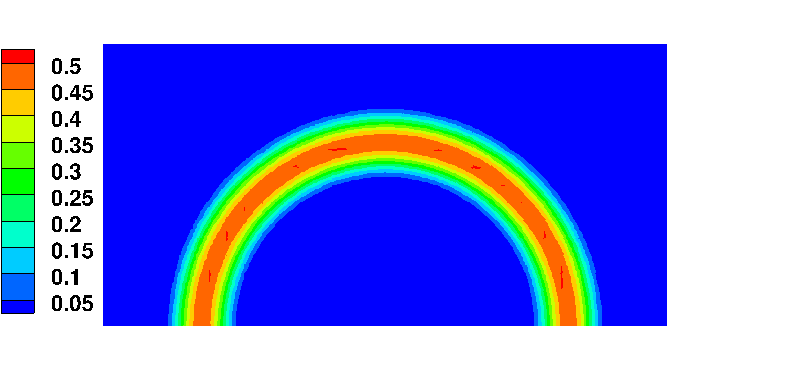
\includegraphics[width=\textwidth, trim = 0mm 15mm 45mm 15mm, clip]
{FIGS/CircularConvection_p=2_lev=4_D=0.png}
\end{minipage}
\begin{minipage}[H]{0.3\textwidth}
\centering
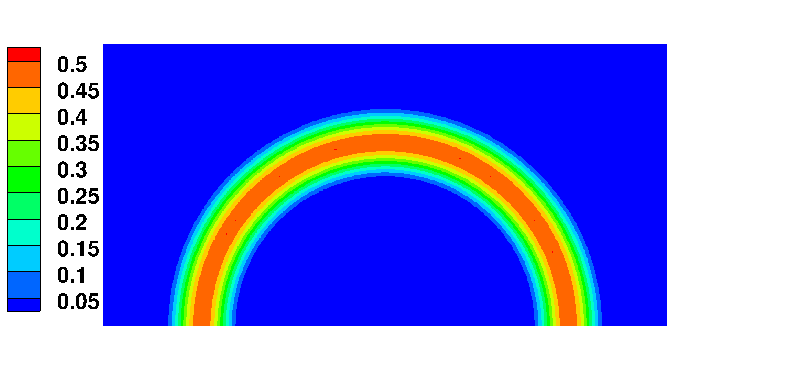
\includegraphics[width=\textwidth, trim = 45mm 15mm 44mm 15mm, clip]
{FIGS/CircularConvection_p=2_lev=5_D=0.png}
\end{minipage}	
\begin{minipage}[H]{0.3\textwidth}
\centering
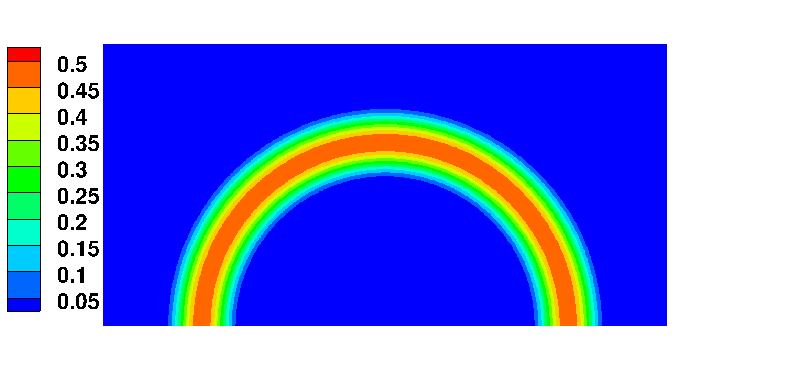
\includegraphics[width=\textwidth, trim = 45mm 15mm 44mm 15mm, clip]
{FIGS/CircularConvection_p=2_lev=6_D=0.png}
\end{minipage}
\vspace{-3mm}
\caption{Circular convection problem with no diffusion, solution using exact linear solver for 
mesh levels 4, 5, and 6 (left to right).}
\label{CC1}
\end{figure}
\begin{figure}[h!]
\vspace{-6mm}
\centering
\begin{minipage}[H]{0.37\textwidth}
\centering
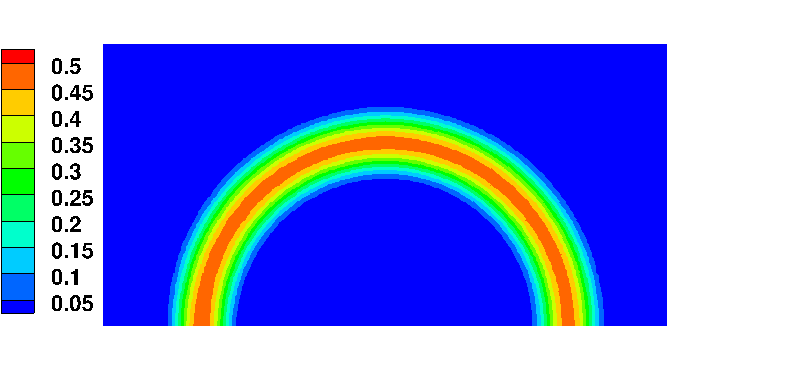
\includegraphics[width=\textwidth, trim = 0mm 15mm 45mm 15mm, clip]
{FIGS/CircularConvection_p=2_lev=4_D=1e-3.png}
 \end{minipage}
\begin{minipage}[H]{0.3\textwidth}
\centering
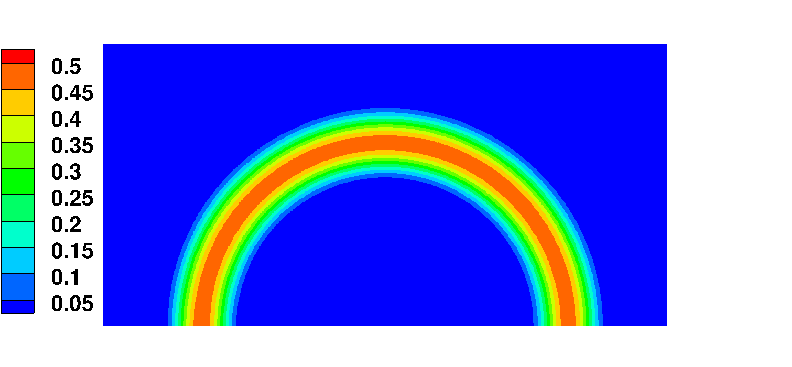
\includegraphics[width=\textwidth, trim = 45mm 15mm 44mm 15mm, clip]
{FIGS/CircularConvection_p=2_lev=5_D=1e-3.png}
\end{minipage}	
\begin{minipage}[H]{0.3\textwidth}
\centering
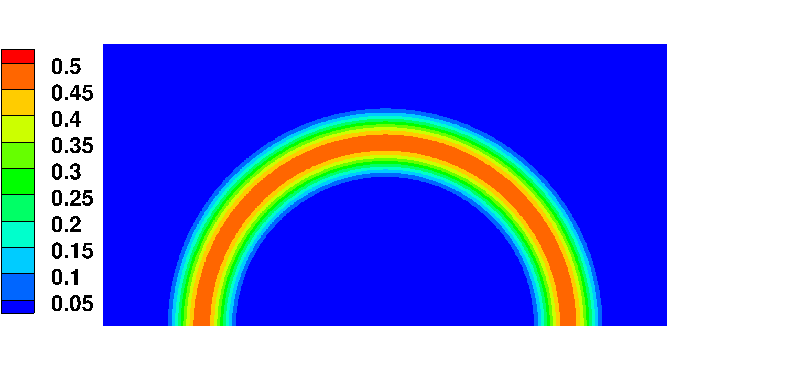
\includegraphics[width=\textwidth, trim = 45mm 15mm 44mm 15mm, clip]
{FIGS/CircularConvection_p=2_lev=6_D=1e-3.png}
\end{minipage}
\vspace{-3mm}
\caption{Circular convection problem with small diffusion $D=0.001$, solution using exact linear solver for 
mesh levels 4, 5, and 6 (left to right).}
\label{CC2}
\end{figure}
\begin{figure}[h!]
\vspace{-6mm}
\centering
\begin{minipage}[H]{0.37\textwidth}
\centering
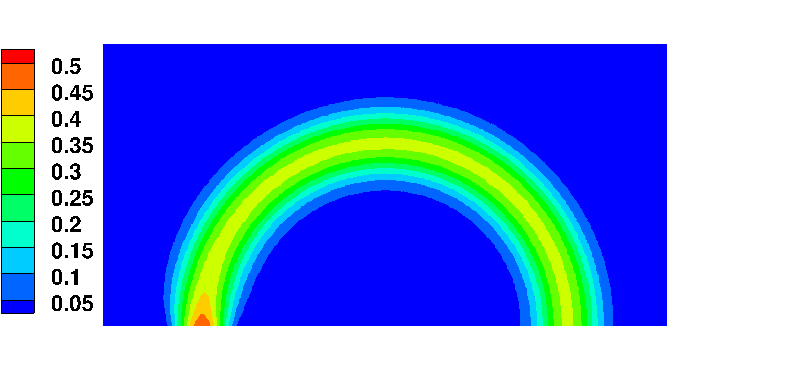
\includegraphics[width=\textwidth, trim = 0mm 15mm 45mm 15mm, clip]
{FIGS/CircularConvection_p=2_lev=4_D=1e-2.png}
\end{minipage}
\begin{minipage}[H]{0.3\textwidth}
\centering
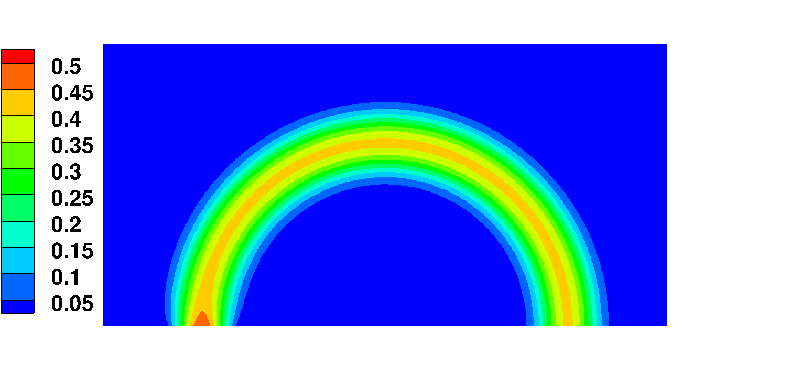
\includegraphics[width=\textwidth, trim = 45mm 15mm 44mm 15mm, clip]
{FIGS/CircularConvection_p=2_lev=5_D=1e-2.png}
\end{minipage}	
\begin{minipage}[H]{0.3\textwidth}
\centering
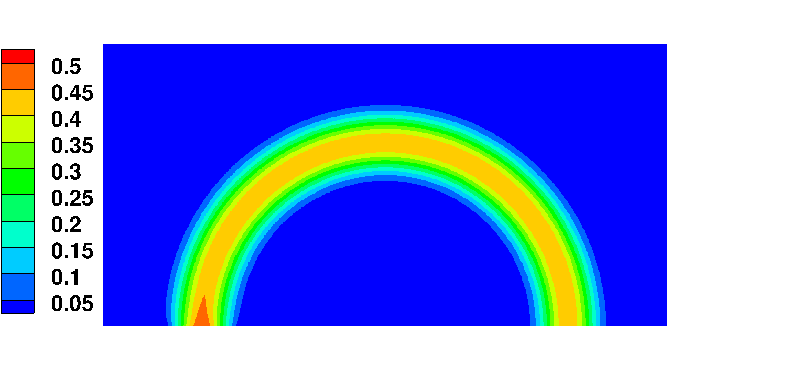
\includegraphics[width=\textwidth, trim = 45mm 15mm 44mm 15mm, clip]
{FIGS/CircularConvection_p=2_lev=6_D=1e-2.png}
\end{minipage}
\vspace{-3mm}
\caption{Circular convection problem with large diffusion $D=0.01$, solution using exact linear solver for 
mesh levels 4, 5, and 6 (left to right).}
\label{CC3}
\end{figure}
\end{frame}



\subsection{Performance comparison - circular convection}

\begin{frame}

{\large Performance comparison HSS vs. p-multigrid -- denoted as MG (number of pre- and postsmoothing iterations)}
\begin{itemize}
\item circular convection problem with no diffusion $D=0$
\item \vspace{-2mm}All tests use piecewise quadratic DG approximation
\item \vspace{-2mm}'CPU' gives the total CPU time in seconds
\item \vspace{-2mm}'Iter.' contains the number of full iterations of the linear solver (V-cycles in the case of the $p$-multigrid method)
\end{itemize}
\begin{minipage}{.45\textwidth}
\small
\begin{table}[h!]
\setlength{\tabcolsep}{2.5pt}
\begin{tabular}{|c|c|c|c|c|c|c|c|c|c|c|}
\hline
\textbf{Grid level} & \multicolumn{2}{c|}{\textbf{3}} & \multicolumn{2}{c|}{\textbf{4}} 
& \multicolumn{2}{c|}{\textbf{5}} & \multicolumn{2}{c|}{\textbf{6}} & \multicolumn{2}{c|}{\textbf{7}} \\ 
\hline
\textbf{Method} & {\textbf{CPU}} & {\textbf{Iter.}} & {\textbf{CPU}}
& {\textbf{Iter.}} & {\textbf{CPU}} & {\textbf{Iter.}}
& {\textbf{CPU}} & {\textbf{Iter.}} & {\textbf{CPU}} & {\textbf{Iter.}} \\ 
\hline
HSS        & 0.24 & 51 & 0.71 & 60 & \ \ 2.42 & 69 &  10.58 & 80 &  42.18 & 71 \\ \hline
$p$-MG(2)  & 0.21 &  5 & 0.87 &  9 & 3.96 & 14 &  19.47 & 21 &  90.56 & 26 \\ \hline
$p$-MG(3)  & 0.21 &  4 & 0.90 &  7 & 4.02 & 10 &  20.59 & 16 & 100.21 & 20 \\ \hline
$p$-MG(5)  & 0.21 &  3 & 0.96 &  5 & 4.39 &  7 &  20.76 & 10 & 108.07 & 14 \\ \hline
$p$-MG(10) & 0.22 &  2 & 1.01 &  3 & 4.71 &  4 &  23.32 &  6 & 131.95 &  9 \\ \hline
$p$-MG(15) & 0.22 &  1 & 1.02 &  2 & 5.10 &  3 &  27.50 &  5 & 134.79 &  6 \\ \hline
\end{tabular}
\label{CC-comp-D=0}
\end{table}
\normalsize
\end{minipage}
\begin{minipage}{.4\textwidth}
\hspace{15mm}
\begin{minipage}{.95\textwidth}
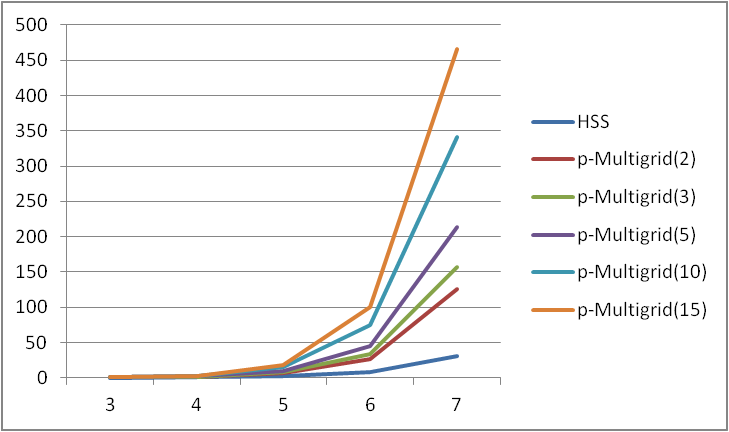
\includegraphics[width=\textwidth]{resultGraphs/circularConvection/comparison1e-1.png}\ \\
{\small {Comparison of HSS with p-Multigrid [CPU time vs. number of grid refinements] with various number of smoothing steps for no diffusion $(D = 0)$.}}
\end{minipage}
\end{minipage}
\end{frame}



\begin{frame}

{\large Performance comparison HSS vs. p-multigrid -- denoted as MG (number of pre- and postsmoothing iterations)}
\begin{itemize}
\item circular convection problem with small diffusion $D=0.001$
\item \vspace{-2mm}All tests use piecewise quadratic DG approximation
\item \vspace{-2mm}'CPU' gives the total CPU time in seconds
\item \vspace{-2mm}'Iter.' contains the number of full iterations of the linear solver (V-cycles in the case of the $p$-multigrid method)
\end{itemize}

\begin{minipage}{.45\textwidth}
\small
\begin{table}[h!]
\setlength{\tabcolsep}{2.5pt}
\begin{tabular}{|c|c|c|c|c|c|c|c|c|c|c|}
\hline
\textbf{Grid level} & \multicolumn{2}{c|}{\textbf{3}} & \multicolumn{2}{c|}{\textbf{4}} 
& \multicolumn{2}{c|}{\textbf{5}} & \multicolumn{2}{c|}{\textbf{6}} & \multicolumn{2}{c|}{\textbf{7}} \\ 
\hline
\textbf{Method} & {\textbf{CPU}} & {\textbf{Iter.}} & {\textbf{CPU}}
& {\textbf{Iter.}} & {\textbf{CPU}} & {\textbf{Iter.}}
& {\textbf{CPU}} & {\textbf{Iter.}} & {\textbf{CPU}} & {\textbf{Iter.}} \\ 
\hline
HSS        & 0.22 & 37 & 0.65 & 44 & \ \ 1.94 & 36 &  6.89 & 28 &  27.47 & 26 \\ \hline
$p$-MG(2)  & 0.23 &  7 & 1.00 & 11 & 4.47 & 19 & 20.83 & 27 &  93.54 & 31 \\ \hline
$p$-MG(3)  & 0.24 &  5 & 0.99 &  8 & 4.68 & 15 & 22.67 & 23 & 107.31 & 29 \\ \hline
$p$-MG(5)  & 0.25 &  4 & 1.03 &  6 & 4.76 & 10 & 25.86 & 19 & 128.89 & 26 \\ \hline
$p$-MG(10) & 0.25 &  2 & 1.03 &  3 & 5.20 &  6 & 32.04 & 13 & 175.85 & 22 \\ \hline
$p$-MG(15) & 0.27 &  2 & 1.13 &  3 & 5.63 &  5 & 34.15 & 10 & 200.29 & 18 \\ \hline
\end{tabular}
\label{CC-comp-D=0.001}
\end{table}
\normalsize
\end{minipage}
\begin{minipage}{.4\textwidth}
\hspace{15mm}
\begin{minipage}{.95\textwidth}
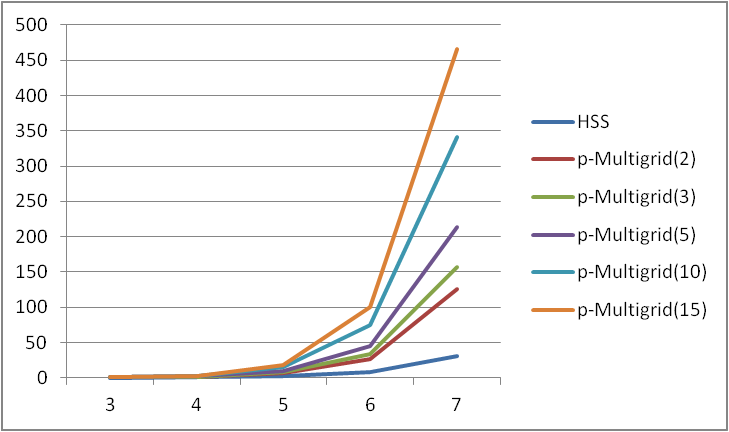
\includegraphics[width=\textwidth]{resultGraphs/circularConvection/comparison1e-1.png}\ \\
{\small {Comparison of HSS with p-Multigrid [CPU time vs. number of grid refinements] with various number of smoothing steps for small diffusion $(D = 10^{-3})$.}} 
\end{minipage}
\end{minipage}
\end{frame}



\begin{frame}

{\large Performance comparison HSS vs. p-multigrid -- denoted as MG (number of pre- and postsmoothing iterations)}
\begin{itemize}
\item circular convection problem with large diffusion $D=0.1$
\item \vspace{-2mm}All tests use piecewise quadratic DG approximation
\item \vspace{-2mm}'CPU' gives the total CPU time in seconds
\item \vspace{-2mm}'Iter.' contains the number of full iterations of the linear solver (V-cycles in the case of the $p$-multigrid method)
\end{itemize}

\begin{minipage}{.45\textwidth}
\small
\begin{table}[h!]
\setlength{\tabcolsep}{2.5pt}
\begin{tabular}{|c|c|c|c|c|c|c|c|c|c|c|}
\hline
\textbf{Grid level} & \multicolumn{2}{c|}{\textbf{3}} & \multicolumn{2}{c|}{\textbf{4}} 
& \multicolumn{2}{c|}{\textbf{5}} & \multicolumn{2}{c|}{\textbf{6}} & \multicolumn{2}{c|}{\textbf{7}} \\ 
\hline
\textbf{Method} & {\textbf{CPU}} & {\textbf{Iter.}} & {\textbf{CPU}}
& {\textbf{Iter.}} & {\textbf{CPU}} & {\textbf{Iter.}}
& {\textbf{CPU}} & {\textbf{Iter.}} & {\textbf{CPU}} & {\textbf{Iter.}} \\ 
\hline
HSS        & 0.16 & 34 & 0.57 & 33 &  1.90 & 33 &  7.36 & 33 &  31.31 & 34 \\ \hline
$p$-MG(2)  & 0.31 & 26 & 1.42 & 41 &  6.31 & 51 & 27.02 & 57 & 125.95 & 61 \\ \hline
$p$-MG(3)  & 0.32 & 22 & 1.60 & 37 &  7.73 & 49 & 33.10 & 56 & 157.37 & 61 \\ \hline
$p$-MG(5)  & 0.36 & 18 & 1.92 & 32 &  9.85 & 45 & 44.62 & 54 & 213.45 & 60 \\ \hline
$p$-MG(10) & 0.42 & 13 & 2.57 & 26 & 14.76 & 40 & 74.56 & 51 & 340.49 & 58 \\ \hline
$p$-MG(15) & 0.47 & 11 & 3.02 & 22 & 18.28 & 36 & 99.76 & 48 & 466.23 & 57 \\ \hline
\end{tabular}
\label{CC-comp-D=0.01}
\end{table}
\normalsize
\end{minipage}
\begin{minipage}{.4\textwidth}
\hspace{15mm}
\begin{minipage}{.95\textwidth}
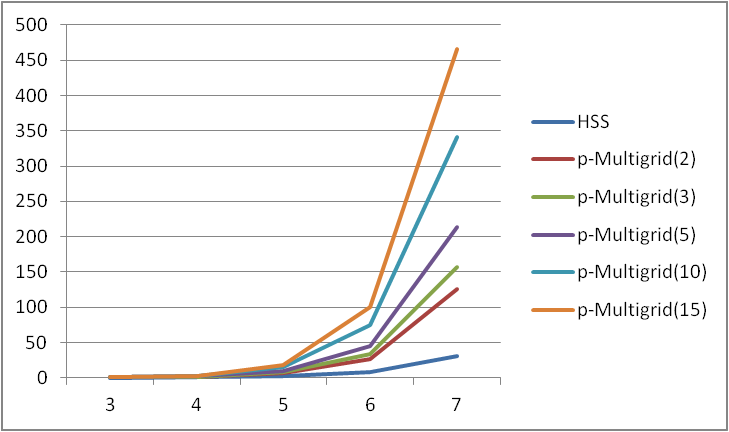
\includegraphics[width=\textwidth]{resultGraphs/circularConvection/comparison1e-1.png}\ \\
{\small {Comparison of HSS with p-Multigrid [CPU time vs. number of grid refinements] with various number of smoothing steps for large diffusion $(D = 10^{-1})$.}}
\end{minipage}
\end{minipage}
\end{frame}

\begin{frame}

{\large Convergence analysis of HSS}
\begin{itemize}
\item circular convection problem with no diffusion $D=0$
\item \vspace{-2mm}All tests use piecewise quadratic DG approximation
\end{itemize}
\begin{figure}
\centering
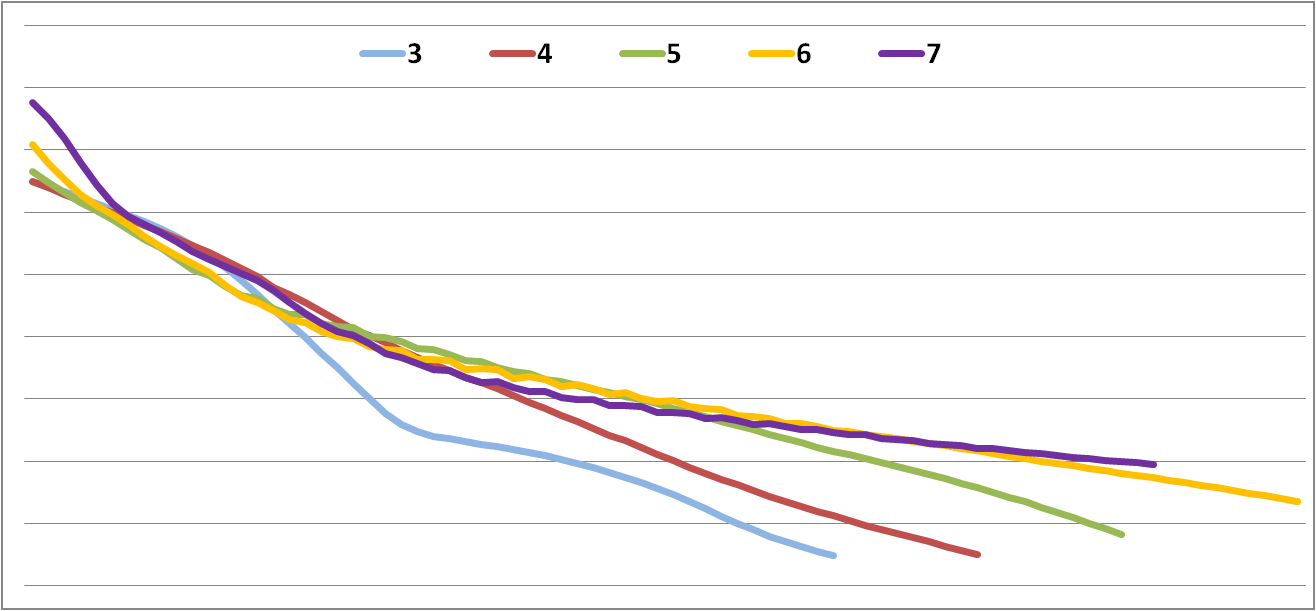
\includegraphics[width=0.7\textwidth]{resultGraphs/circularConvection/p2D0_new.png}
\end{figure}
\end{frame}

\begin{frame}

{\large Convergence analysis of HSS}
\begin{itemize}
\item circular convection problem with small diffusion $D=0.001$
\item \vspace{-2mm}All tests use piecewise quadratic DG approximation
\end{itemize}
\begin{figure}
\centering
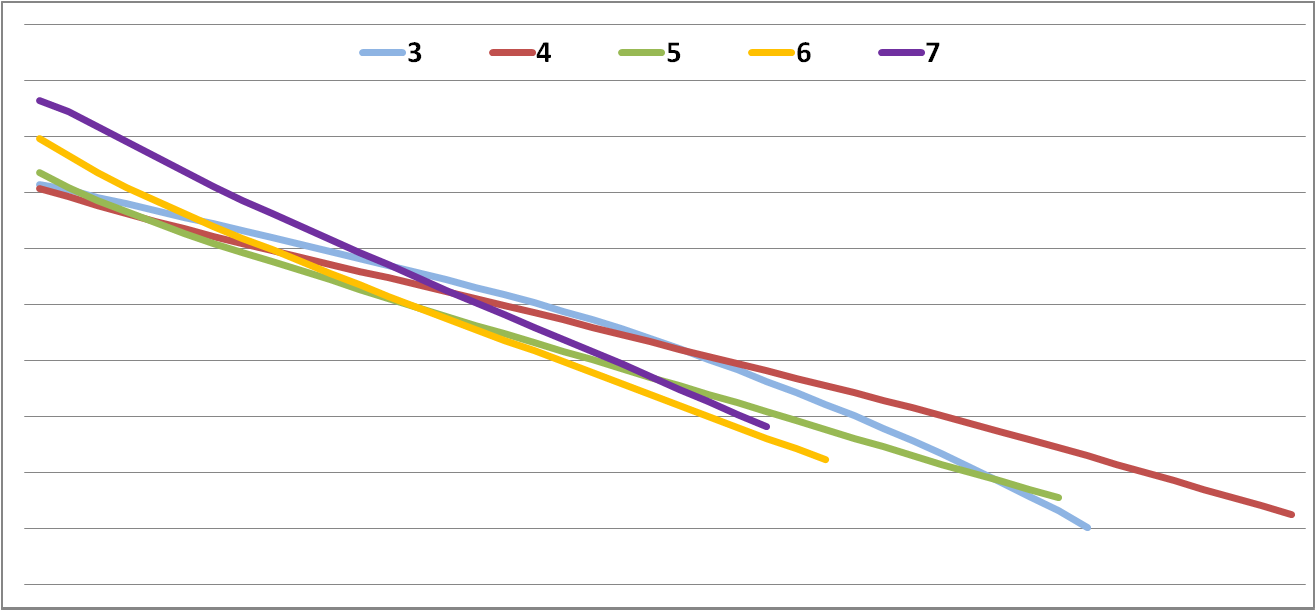
\includegraphics[width=0.7\textwidth]{resultGraphs/circularConvection/p2D1e-3_new.png}
\end{figure}
\end{frame}

\begin{frame}

{\large Convergence analysis of HSS}
\begin{itemize}
\item circular convection problem with large diffusion $D=0.1$
\item \vspace{-2mm}All tests use piecewise quadratic DG approximation
\end{itemize}
\begin{figure}
\centering
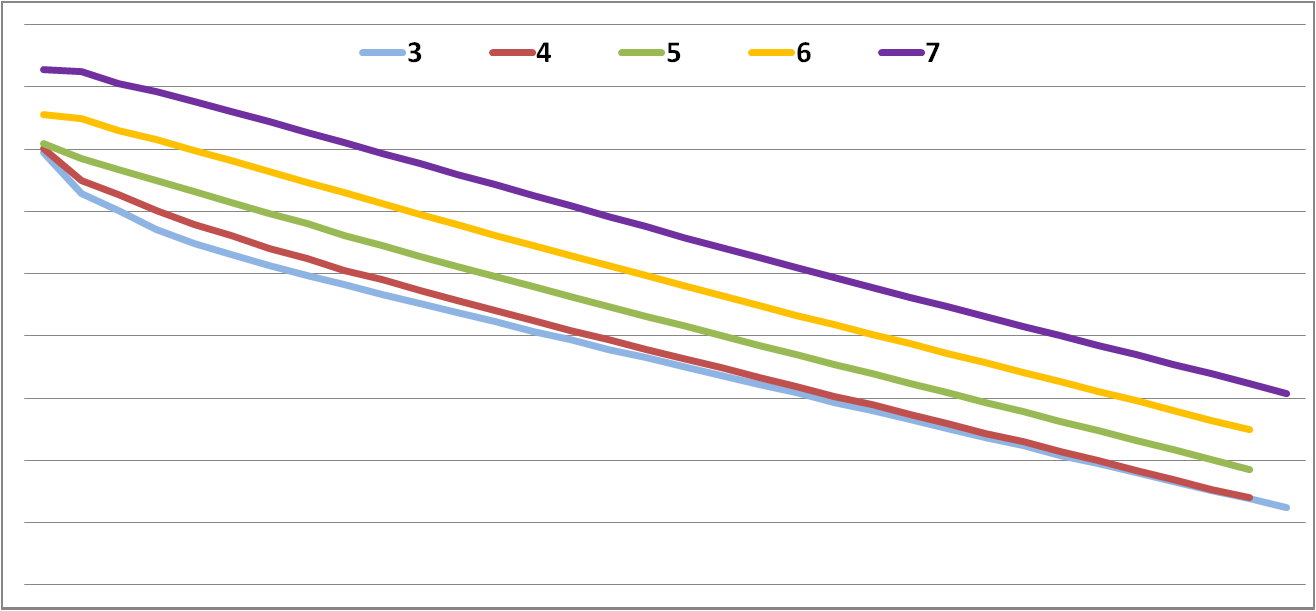
\includegraphics[width=0.7\textwidth]{resultGraphs/circularConvection/p2D1e-1_new.png}
\end{figure}
\end{frame}


\subsection{Rotating peak}
\begin{frame}
In the second test case, the time-dependent transport equation (\ref{goveq}) 
with
$$\ba(x,y)=(-y,x),\qquad D=10^{-2}$$
is solved in the square domain $\Omega=(-1,1)\times(-1,1)$. The time interval
of interest is $\left[\frac{\pi}{2}, \frac{5\pi}{2}\right]$. The exact
solution, inflow boundary conditions, and the initial solution at
$t_0=\frac{\pi}{2}$ are given by the formula
\begin{equation}
u(x,y)=
\frac{1}{4\pi D t}\exp\left({\frac{-r^2}{4 D t}}\right),
\label{rotating-peak-data}
\end{equation}
where $r=\sqrt{x^2+y^2}$ is the distance from the center $(0.0,0.0)$. 
Homogeneous Neumann boundary conditions are
prescribed on all outflow boundaries. 
\begin{figure}[H]
\centering
	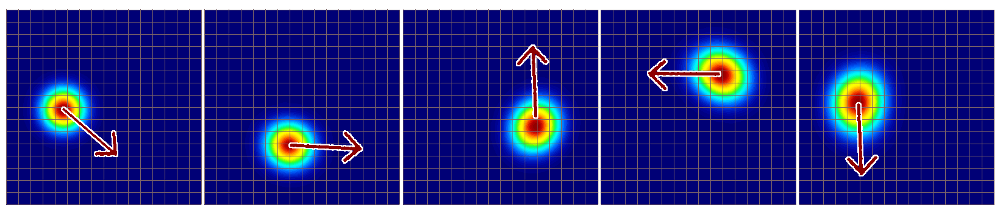
\includegraphics[width=.75\textwidth]{images/timedep.png}
\end{figure}

\end{frame}

\begin{frame}
First, we are interested in stability of the HSS method; we ran the example for various CFL numbers:
%CFL=0.25
\begin{figure}[H]
\centering
	\begin{subfigure}[H]{0.02\textwidth}
		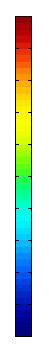
\includegraphics[width=\textwidth]{images/timedep-multiscale/stability/scale.jpg}
	\end{subfigure}
	\begin{subfigure}[H]{0.3\textwidth}
	\centering
		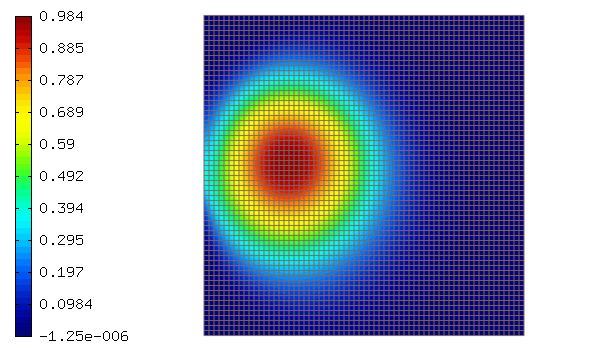
\includegraphics[width=.9\textwidth, trim = 65mm 0mm 0mm 0mm, clip]{images/timedep-multiscale/stability/eps=001_804.jpg}
		\vspace{-3mm}
		\caption{$D = 10^{-2}$\\\vspace{-2mm}scale [0; 0.984]}
	\end{subfigure}
	\begin{subfigure}[H]{0.3\textwidth}
	\centering
		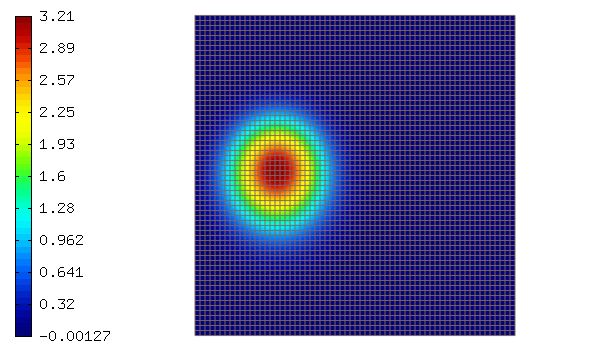
\includegraphics[width=.9\textwidth, trim = 65mm 0mm 0mm 0mm, clip]{images/timedep-multiscale/stability/eps=0001_804.jpg}
		\vspace{-3mm}
		\caption{$D = 10^{-3}$\\\vspace{-2mm}scale [-0.00127; 3.21]}
	\end{subfigure}
	\begin{subfigure}[H]{0.3\textwidth}
	\centering
		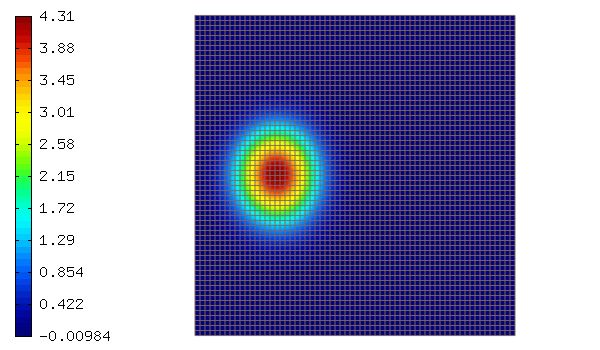
\includegraphics[width=.9\textwidth, trim = 65mm 0mm 0mm 0mm, clip]{images/timedep-multiscale/stability/eps=0_804.jpg}
		\vspace{-3mm}
		\caption{$D = 0$\\\vspace{-2mm}scale [-0.00984; 4.31]}
	\end{subfigure}
	\vspace{-3mm}
	\caption{Solution after one rotation, $CFL = 0.25$}	
\end{figure}
\vspace{-8mm}
%CFL=0.5
\begin{figure}[H]
\centering
	\begin{subfigure}[H]{0.02\textwidth}
		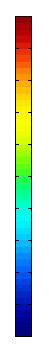
\includegraphics[width=\textwidth]{images/timedep-multiscale/stability/scale.jpg}
	\end{subfigure}
	\begin{subfigure}[H]{0.3\textwidth}
		\centering
		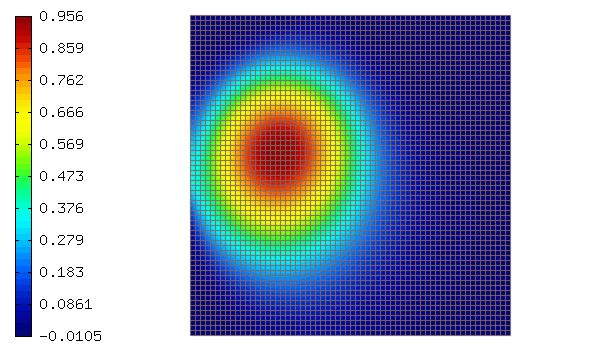
\includegraphics[width=.9\textwidth, trim = 65mm 0mm 0mm 0mm, clip]{images/timedep-multiscale/stability/eps=001_402.jpg}
		\vspace{-3mm}
		\caption{$D = 10^{-2}$\\\vspace{-2mm}scale [-0.0105; 0.956]}
	\end{subfigure}
	\begin{subfigure}[H]{0.3\textwidth}
		\centering
		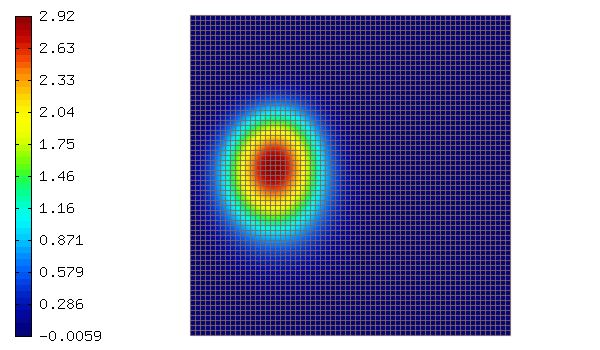
\includegraphics[width=.9\textwidth, trim = 65mm 0mm 0mm 0mm, clip]{images/timedep-multiscale/stability/eps=0001_402.jpg}
		\vspace{-3mm}
		\caption{$D = 10^{-3}$\\\vspace{-2mm}scale [-0.0059; 2.92]}
	\end{subfigure}
	\begin{subfigure}[H]{0.3\textwidth}
		\centering
		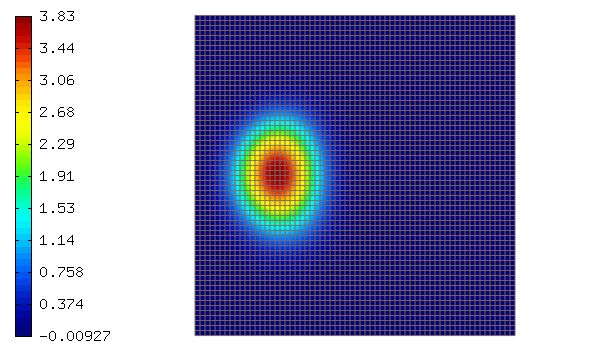
\includegraphics[width=.9\textwidth, trim = 65mm 0mm 0mm 0mm, clip]{images/timedep-multiscale/stability/eps=0_402.jpg}
		\vspace{-3mm}
		\caption{$D = 0$\\\vspace{-2mm}scale [-0.00927; 3.83]}
	\end{subfigure}
	\vspace{-3mm}
	\caption{Solution after one rotation, $CFL = 0.5$}	
\end{figure}

\end{frame}



\begin{frame}
First, we are interested in stability of the HSS method; we ran the example for various CFL numbers:
\begin{figure}[H]
\centering
	\begin{subfigure}[H]{0.02\textwidth}
		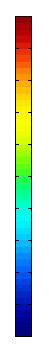
\includegraphics[width=\textwidth]{images/timedep-multiscale/stability/scale.jpg}
	\end{subfigure}
	\begin{subfigure}[H]{0.3\textwidth}
		\centering
		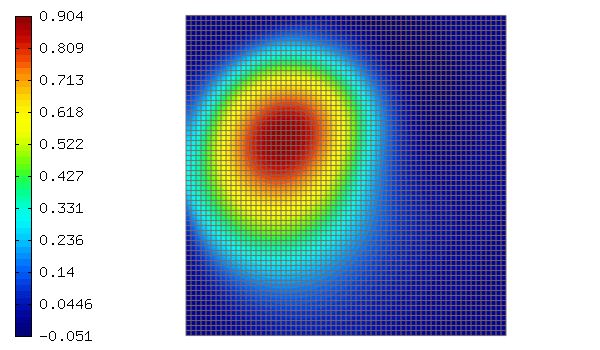
\includegraphics[width=.9\textwidth, trim = 65mm 0mm 0mm 0mm, clip]{images/timedep-multiscale/stability/eps=001_201.jpg}
		\vspace{-3mm}
		\caption{$D = 10^{-2}$\\\vspace{-2mm}scale [-0.051; .904]}
	\end{subfigure}
	\begin{subfigure}[H]{0.3\textwidth}
		\centering
		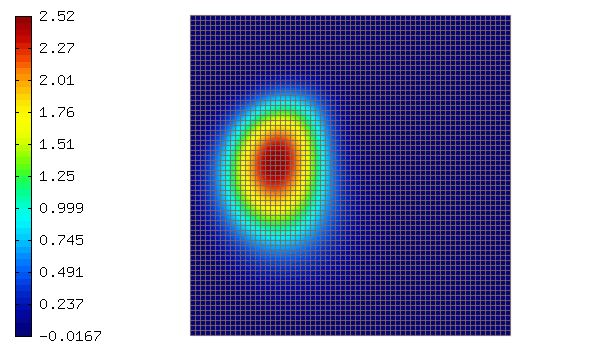
\includegraphics[width=.9\textwidth, trim = 65mm 0mm 0mm 0mm, clip]{images/timedep-multiscale/stability/eps=0001_201.jpg}
		\vspace{-3mm}
		\caption{$D = 10^{-3}$\\\vspace{-2mm}scale [-0.0167; 2.52]}
	\end{subfigure}
	\begin{subfigure}[H]{0.3\textwidth}
		\centering
		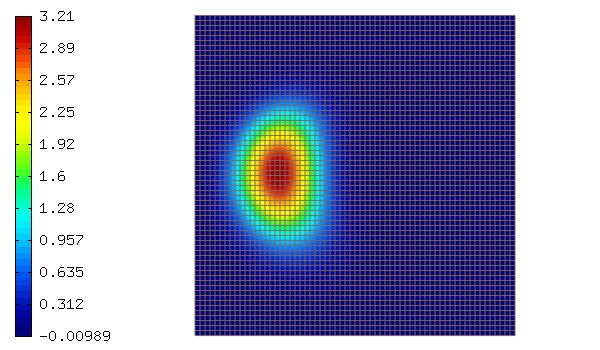
\includegraphics[width=.9\textwidth, trim = 65mm 0mm 0mm 0mm, clip]{images/timedep-multiscale/stability/eps=0_201.jpg}
		\vspace{-3mm}
		\caption{$D = 0$\\\vspace{-2mm}scale [-0.00989; 3.21]}
	\end{subfigure}
	\vspace{-3mm}
	\caption{Solution after one rotation, $CFL = 1.0$}	
\end{figure}
\vspace{-8mm}
%CFL=2
\begin{figure}[H]
\centering
	\begin{subfigure}[H]{0.02\textwidth}
		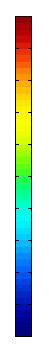
\includegraphics[width=\textwidth]{images/timedep-multiscale/stability/scale.jpg}
	\end{subfigure}
	\begin{subfigure}[H]{0.3\textwidth}
		\centering
		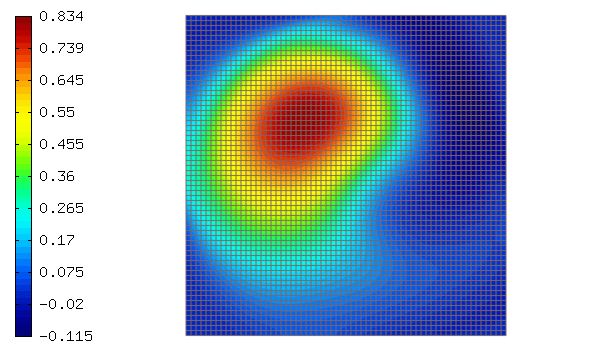
\includegraphics[width=.9\textwidth, trim = 65mm 0mm 0mm 0mm, clip]{images/timedep-multiscale/stability/eps=001_100.jpg}
		\vspace{-3mm}
		\caption{$D = 10^{-2}$\\\vspace{-2mm}scale [-0.115; .834]}
	\end{subfigure}
	\begin{subfigure}[H]{0.3\textwidth}
		\centering
		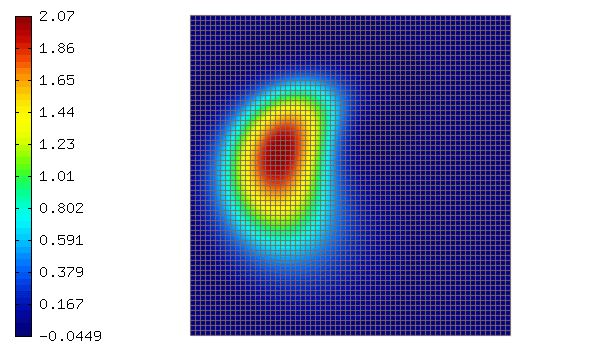
\includegraphics[width=.9\textwidth, trim = 65mm 0mm 0mm 0mm, clip]{images/timedep-multiscale/stability/eps=0001_100.jpg}
		\vspace{-3mm}
		\caption{$D = 10^{-3}$\\\vspace{-2mm}scale [-0.0449; 2.07]}
	\end{subfigure}
	\begin{subfigure}[H]{0.3\textwidth}
		\centering
		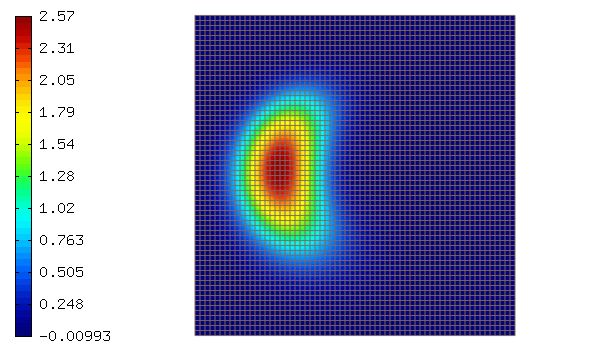
\includegraphics[width=.9\textwidth, trim = 65mm 0mm 0mm 0mm, clip]{images/timedep-multiscale/stability/eps=0_100.jpg}
		\vspace{-3mm}
		\caption{$D = 0$\\\vspace{-2mm}scale [-0.00993; 2.57]}
	\end{subfigure}
	\vspace{-3mm}
	\caption{Solution after one rotation, $CFL = 2.0$}	
\end{figure}

\end{frame}



\begin{frame}
First, we are interested in stability of the HSS method; we ran the example for various CFL numbers:
\begin{figure}[H]
\centering
	\begin{subfigure}[H]{0.02\textwidth}
		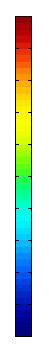
\includegraphics[width=\textwidth]{images/timedep-multiscale/stability/scale.jpg}
	\end{subfigure}
	\begin{subfigure}[H]{0.3\textwidth}
		\centering
		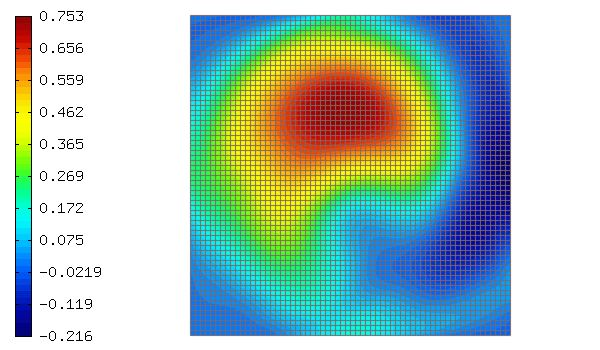
\includegraphics[width=.9\textwidth, trim = 65mm 0mm 0mm 0mm, clip]{images/timedep-multiscale/stability/eps=001_50.jpg}
		\vspace{-3mm}
		\caption{$D = 10^{-2}$\\\vspace{-2mm}scale [-0.216; 0.753]}
	\end{subfigure}
	\begin{subfigure}[H]{0.3\textwidth}
		\centering
		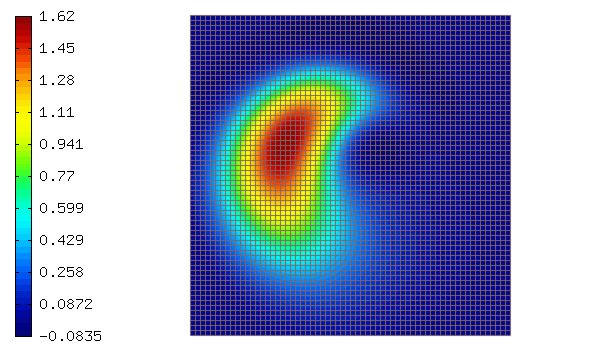
\includegraphics[width=.9\textwidth, trim = 65mm 0mm 0mm 0mm, clip]{images/timedep-multiscale/stability/eps=0001_50.jpg}
		\vspace{-3mm}
		\caption{$D = 10^{-3}$\\\vspace{-2mm}scale [-0.0835; 1.62]}
	\end{subfigure}
	\begin{subfigure}[H]{0.3\textwidth}
		\centering
		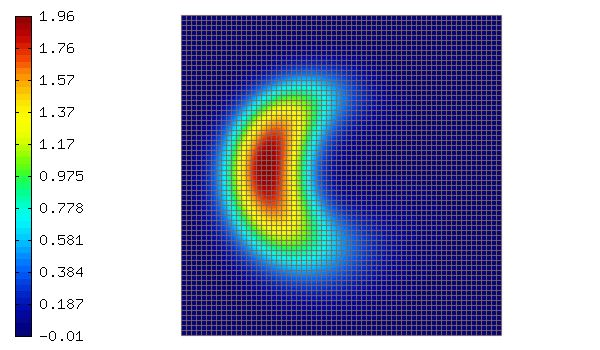
\includegraphics[width=.9\textwidth, trim = 65mm 0mm 0mm 0mm, clip]{images/timedep-multiscale/stability/eps=0_50.jpg}
		\vspace{-3mm}
		\caption{$D = 0$\\\vspace{-2mm}scale \emph{}[-0.01; 1.96]}
	\end{subfigure}
	\vspace{-3mm}
	\caption{Solution after one rotation, $CFL = 4.0$}	
\end{figure}
\noindent



We can see that the solution is stable for $CFL = 4.0$, but for convergence investigation, we have to use smaller $CFL$ for accuracy reasons.


\end{frame}



\begin{frame}
Taking a look at the convergence, we present the results for various values of the diffusivity coefficient, and $CFL=1.0$.
\begin{figure}[H]
\centering
	\begin{subfigure}[H]{0.02\textwidth}
		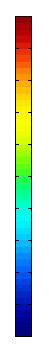
\includegraphics[width=\textwidth]{images/timedep-multiscale/stability/scale.jpg}
	\end{subfigure}
	\begin{subfigure}[H]{0.3\textwidth}
		\centering
		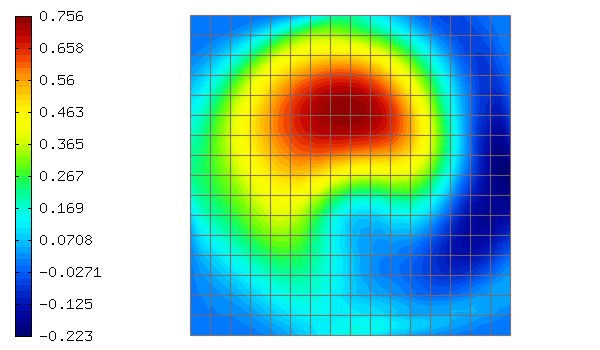
\includegraphics[width=.9\textwidth, trim = 65mm 0mm 0mm 0mm, clip]{images/timedep-multiscale/convergence/256_eps=001_50.jpg}
		\vspace{-3mm}
		\caption{$D = 10^{-2}$\\\vspace{-2mm}scale [-0.223; 0.756]}
	\end{subfigure}
	\begin{subfigure}[H]{0.3\textwidth}
		\centering
		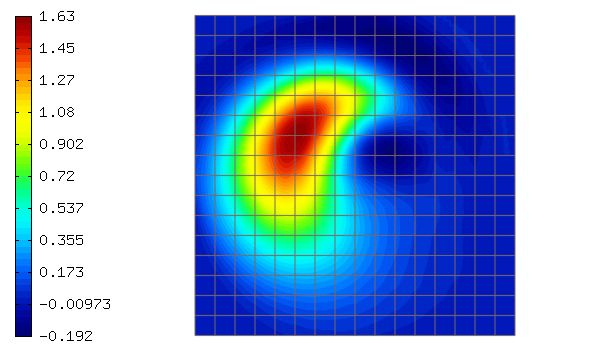
\includegraphics[width=.9\textwidth, trim = 65mm 0mm 0mm 0mm, clip]{images/timedep-multiscale/convergence/256_eps=0001_50.jpg}
		\vspace{-3mm}
		\caption{$D = 10^{-3}$\\\vspace{-2mm}scale [-0.192; 1.63]}
	\end{subfigure}
	\begin{subfigure}[H]{0.3\textwidth}
		\centering
		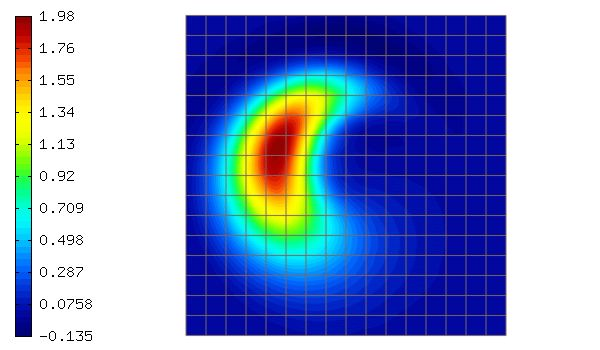
\includegraphics[width=.9\textwidth, trim = 65mm 0mm 0mm 0mm, clip]{images/timedep-multiscale/convergence/256_eps=0_50.jpg}
		\vspace{-3mm}
		\caption{$D = 0$\\\vspace{-2mm}scale [-0.135; 1.98]}
	\end{subfigure}
	\vspace{-3mm}
	\caption{Solution after one rotation, 4 uniform mesh refinements}	
\end{figure}
\vspace{-8mm}
\begin{figure}[H]
\centering
	\begin{subfigure}[H]{0.02\textwidth}
		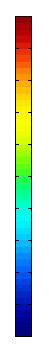
\includegraphics[width=\textwidth]{images/timedep-multiscale/stability/scale.jpg}
	\end{subfigure}
	\begin{subfigure}[H]{0.3\textwidth}
		\centering
		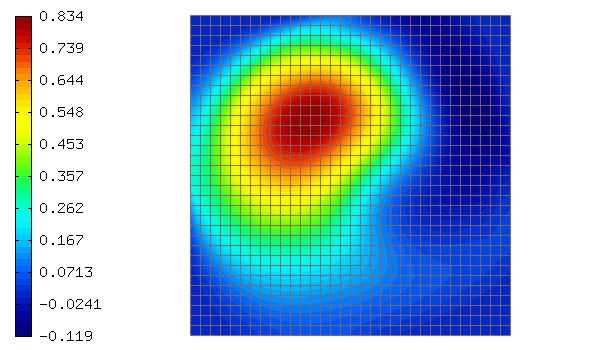
\includegraphics[width=.9\textwidth, trim = 65mm 0mm 0mm 0mm, clip]{images/timedep-multiscale/convergence/1024_eps=001_100.jpg}
		\vspace{-3mm}
		\caption{$D = 10^{-2}$\\\vspace{-2mm}scale [-0.119; 0.834]}
	\end{subfigure}
	\begin{subfigure}[H]{0.3\textwidth}
		\centering
		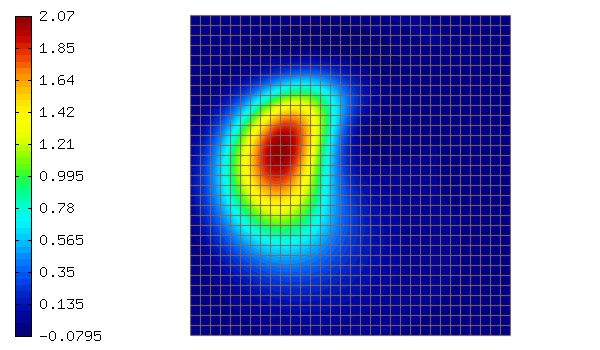
\includegraphics[width=.9\textwidth, trim = 65mm 0mm 0mm 0mm, clip]{images/timedep-multiscale/convergence/1024_eps=0001_100.jpg}
		\vspace{-3mm}
		\caption{$D = 10^{-3}$\\\vspace{-2mm}scale [-0.0795; 2.07]}
	\end{subfigure}
	\begin{subfigure}[H]{0.3\textwidth}
		\centering
		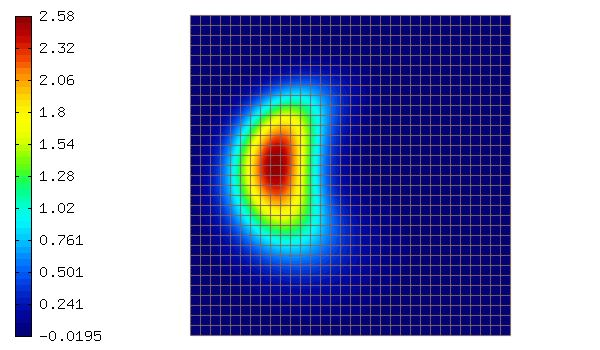
\includegraphics[width=.9\textwidth, trim = 65mm 0mm 0mm 0mm, clip]{images/timedep-multiscale/convergence/1024_eps=0_100.jpg}
		\vspace{-3mm}
		\caption{$D = 0$\\\vspace{-2mm}scale [-0.0195; 2.58]}
	\end{subfigure}
	\vspace{-3mm}
	\caption{Solution after one rotation, 5 uniform mesh refinements}	
\end{figure}

\end{frame}



\begin{frame}
Taking a look at the convergence, we present the results for various values of the diffusivity coefficient, and $CFL=1.0$.
\begin{figure}[H]
\centering
	\begin{subfigure}[H]{0.02\textwidth}
		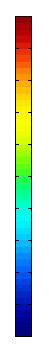
\includegraphics[width=\textwidth]{images/timedep-multiscale/stability/scale.jpg}
	\end{subfigure}
	\begin{subfigure}[H]{0.3\textwidth}
		\centering
		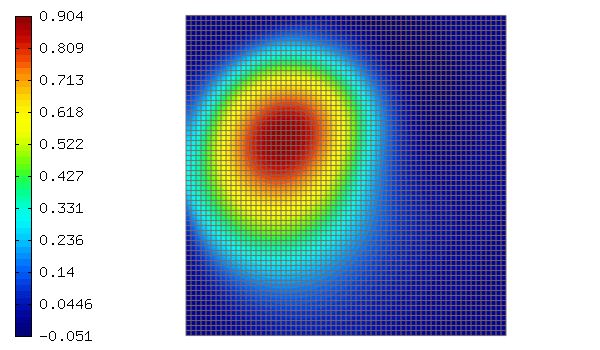
\includegraphics[width=.9\textwidth, trim = 65mm 0mm 0mm 0mm, clip]{images/timedep-multiscale/convergence/4096_eps=001_201.jpg}
		\vspace{-3mm}
		\caption{$D = 10^{-2}$\\\vspace{-2mm}scale [-0.051; .904]}
	\end{subfigure}
	\begin{subfigure}[H]{0.3\textwidth}
		\centering
		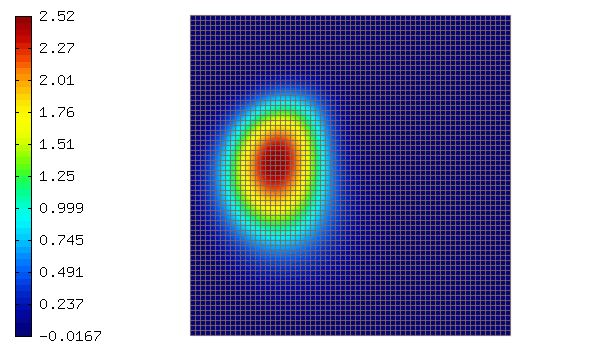
\includegraphics[width=.9\textwidth, trim = 65mm 0mm 0mm 0mm, clip]{images/timedep-multiscale/convergence/4096_eps=0001_201.jpg}
		\vspace{-3mm}
		\caption{$D = 10^{-3}$\\\vspace{-2mm}scale [-0.0167; 2.52]}
	\end{subfigure}
	\begin{subfigure}[H]{0.3\textwidth}
		\centering
		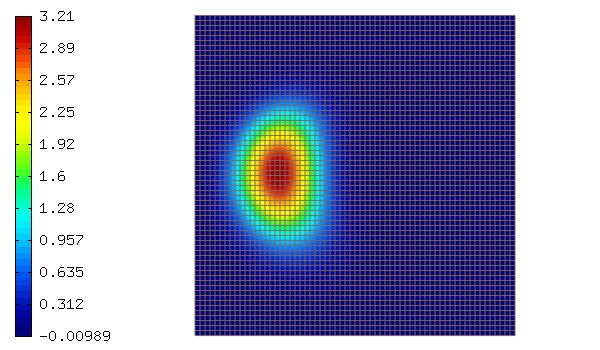
\includegraphics[width=.9\textwidth, trim = 65mm 0mm 0mm 0mm, clip]{images/timedep-multiscale/convergence/4096_eps=0_201.jpg}
		\vspace{-3mm}
		\caption{$D = 0$\\\vspace{-2mm}scale [-0.00989; 3.21]}
	\end{subfigure}
	\vspace{-3mm}
	\caption{Solution after one rotation, 6 uniform mesh refinements}	
\end{figure}
\vspace{-8mm}
\begin{figure}[H]
\centering
	\begin{subfigure}[H]{0.02\textwidth}
		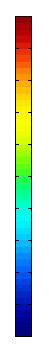
\includegraphics[width=\textwidth]{images/timedep-multiscale/stability/scale.jpg}
	\end{subfigure}
	\begin{subfigure}[H]{0.3\textwidth}
		\centering
		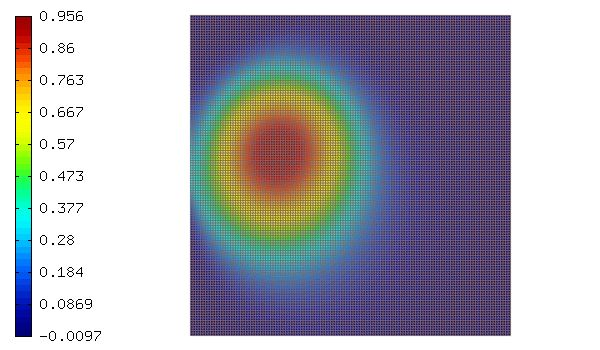
\includegraphics[width=.9\textwidth, trim = 65mm 0mm 0mm 0mm, clip]{images/timedep-multiscale/convergence/16384_eps=001_402.jpg}
		\vspace{-3mm}
		\caption{$D = 10^{-2}$\\\vspace{-2mm}scale [-0.0097; 0.956]}
	\end{subfigure}
	\begin{subfigure}[H]{0.3\textwidth}
		\centering
		\includegraphics[width=.9\textwidth, trim = 65mm 0mm 0mm 0mm, clip]{images/timedep-multiscale/convergence/16384_eps=0001_402.jpg}
		\vspace{-3mm}
		\caption{$D = 10^{-3}$\\\vspace{-2mm}scale [-0.00362; 2.92]}
	\end{subfigure}
	\begin{subfigure}[H]{0.3\textwidth}
		\centering
		\includegraphics[width=.9\textwidth, trim = 65mm 0mm 0mm 0mm, clip]{images/timedep-multiscale/convergence/16384_eps=0_402.jpg}
		\vspace{-3mm}
		\caption{$D = 0$\\\vspace{-2mm}scale [-0.00812; 3.82]}
	\end{subfigure}
	\vspace{-3mm}
	\caption{Solution after one rotation, 7 uniform mesh refinements}	
\end{figure}

\end{frame}

\begin{frame}
\vspace{5mm}
\centering
{\Huge Outlook}\ \\
\begin{itemize}
\item test the method on the Euler and the full Navier-Stokes equations
\item test nonlinear cases
\item test on real examples (in 3D ocean modelling)
\end{itemize}
\vspace{6mm}
\noindent\rule{8cm}{0.4pt}

\vspace{8mm}
{\Huge Thank you for your attention.}

\end{frame}


\end{document}